\section{Data}
\label{sec:data}

\subsection{\Glsfmtfullpl{gemm}}
\label{sec:mouse_models}
\glsunset{gemm}
Mouse models play a crucial role in breast cancer research, offering a powerful
tool for understanding the molecular mechanisms of disease development and
progression.
\Glspl{gemm} allow researchers to manipulate specific genes, such as those
involved in estrogen signaling\supercite{park_mouse_2018}.
These models can closely mimic human breast cancer, providing insights into the
initiation, progression, and metastasis of tumors in a controlled and
reproducible environment\supercite{pfefferle_transcriptomic_2013}.
Additionally, mouse models enable the study of cancer within the context of a
living organism, allowing for the evaluation of hormonal influences, immune
responses, and interactions with the tumor
microenvironment\supercite{manning_mouse_2016}.
This makes them indispensable for preclinical testing of new therapies,
including hormone-targeting treatments like tamoxifen and aromatase inhibitors,
which are standard in the management of hormone receptor-positive breast
cancer\supercite{fan_endocrine_2015,yin_disruption_2014}.
By studying cancer in mice, researchers can identify potential biomarkers,
refine therapeutic strategies, and deepen our understanding of the pathways
driving breast cancer in humans\supercite{peterson_amphiregulin_2015}.

\subsection{Datasets}
\label{sec:datasets}
The datasets used in this thesis are derived from two complementary studies by
\textcite{furth_esr1_2023,furth_overexpression_2023} that investigate the role
of estrogen signaling in breast cancer through the use of \glspl{gemm}.

One dataset comes from an aging study, which focuses on how the overexpression
of Esr1 (the gene coding for \gls{era}) and CYP19A1 (the gene coding for
aromatase) in mammary epithelial cells influences cancer development as the
mice age past reproductive senescence.
The second dataset originates from an anti-hormonal study, which examines the
effects of tamoxifen and letrozole treatments on \glspl{gemm} during
reproductive senescence.

Both datasets provide critical insights into the molecular mechanisms linking
aging, estrogen signaling, and breast cancer progression.

\subsubsection{Study design}

In both studies, the \glspl{gemm} were modified to overexpress either Esr1 or
CYP19A1 in their mammary epithelial cells when treated with doxycycline.
This genetic manipulation was designed to model increased estrogen signaling,
which is known to be a critical factor in breast cancer development, especially
after menopause\supercite{furth_esr1_2023,furth_overexpression_2023}.
The studies focused on inducing this overexpression at or around reproductive
senescence, which is a model for menopause in women, to better understand the
increased cancer risks in aging mammary
tissue\supercite{furth_esr1_2023,furth_overexpression_2023}.

The timeline of the two studies is illustrated in \cref{fig:dataset_timeline}.

\begin{figure}[ht]
    \centering

    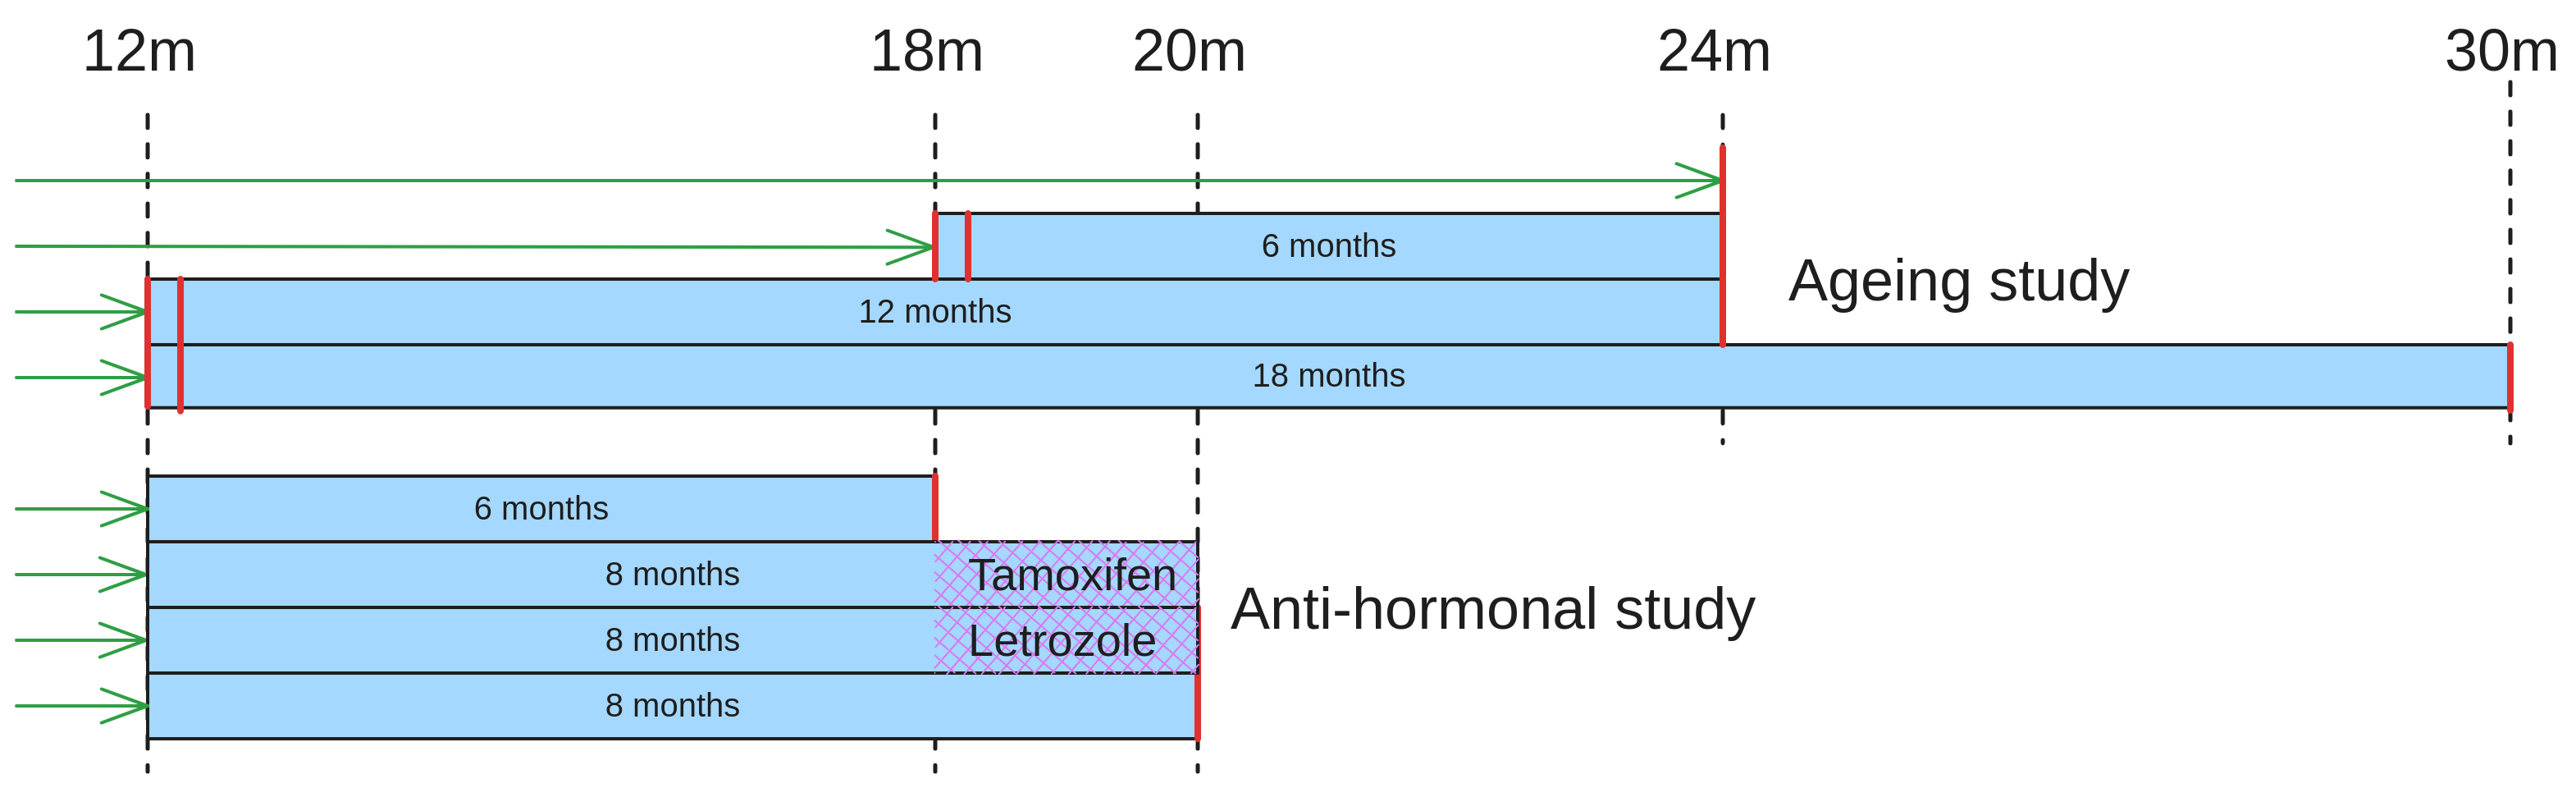
\includegraphics[width=\textwidth]{chapters/3_materials_and_methods/figures/datasets.png}
    \caption{Overview of the two studies and their respective timelines.
        Each red line represents two cohorts of mice that was euthanized for tissue
        collection: one with the Esr1 transgene and one with the CYP19A1 transgene.
        The green arrows indicate periods without transgene induction, while the blue
        blocks indicate the periods of doxycycline treatment to induce the transgenes.
    } \label{fig:dataset_timeline} \end{figure}

\subsubsection{Differences in treatment}
The key difference between the two studies lies in the timing and duration of
the transgene induction, as well as the subsequent treatment with anti-hormonal
therapies.

\paragraph{Anti-hormonal study}
In the anti-hormonal study, eight different cohorts of mice were investigated,
four with the Esr1 transgene and four with the CYP19A1 transgene.
As shown in \cref{fig:dataset_timeline}, the mice were treated with doxycycline
to induce the transgenes at 12 months of age, corresponding to middle age in
humans.

At 18 months of age (6 months of transgene induction), one cohort of each
genotype was euthanized to collect mammary gland tissue as a pre-treatment
control.
At the same time, two cohorts of each genotype were started being treated with
tamoxifen or letrozole, respectively.
The remaining cohort of each genotype was left untreated as a control.

After two more months (now 20 months of age), the remaining three cohorts
(tamoxifen, letrozole, control) of each genotype were
euthanized\supercite{furth_esr1_2023}.

\paragraph{Aging study}
The aging study consists of 16 cohorts of mice, eight with the Esr1 transgene
and eight with the CYP19A1 transgene.
At 12 months of age, one cohort of each genotype was euthanized to collect
mammary gland tissue as a pre-transgene induction control.
For three cohorts of each genotype, the transgene induction was started at 12
months of age.

One of the three cohorts with transgene induction started at 12 months was
euthanized after 1 week of doxycycline treatment to assess the immediate
effects of the transgene induction.
The remaining two cohorts were euthanized at 24 and 30 months of age to
investigate the long-term effects of the transgene induction.

One cohort of each genotype that did not receive the transgene induction was
euthanized at 18 months of age.
Two other cohorts of each genotype started the transgene induction at 18 months
of age.
Of these two cohorts, one was euthanized after 1 week of doxycycline treatment,
while the other was euthanized at 24 months of age.

Lastly, one cohort of each genotype that did not receive any transgene
induction was euthanized at 24 months of
age\supercite{furth_overexpression_2023}.

\subsubsection{Sequencing process} \label{sec:dataset_sequencing}
Both studies used \gls{rna-seq} to analyze gene expression in the mammary
glands.
After euthanasia, thoracic mammary glands were flash frozen, and \gls{rna} was
extracted using a Direct Zol \gls{rna} miniprep kit.
The sequencing libraries were prepared from ribosome-depleted \gls{rna} and
sequenced using the Illumina NextSeq 550 platform with a single-end 75-bp read
length\supercite{furth_esr1_2023,furth_overexpression_2023}.

\subsubsection{Findings}

\paragraph{Anti-hormonal study}
The study found that Esr1 overexpression significantly increased the expression
of genes related to cell proliferation, particularly those linked to poor
prognostic indicators in early-stage hormone receptor-positive breast cancer.
Tamoxifen and letrozole treatments were able to reduce this elevated
proliferative signature, but only Esr1 mice showed substantial responsiveness
to tamoxifen during reproductive senescence.
Both models were responsive to letrozole before and after reproductive
senescence\supercite{furth_esr1_2023}.

\paragraph{Aging study}
This study demonstrated that Esr1 overexpression in aged mice led to a higher
prevalence of estrogen receptor-positive mammary adenocarcinomas.
The tumors in Esr1-overexpressing mice were predominantly \gls{er}-positive,
whereas CYP19A1 mice exhibited a mix of \gls{er}-positive and adenosquamous
carcinomas.
The Esr1 mice developed a persistent proliferative signature similar to that
found in human \gls{er}-positive breast cancer, supporting the role of aging
and prolonged estrogen exposure in the generation of these
cancers\supercite{furth_overexpression_2023}.
